\documentclass[12pt, oneside]{article}
\usepackage{a4wide}
\usepackage{oldgerm}
\usepackage{amsmath}
\usepackage{amssymb}
\usepackage{amstext}
\setlength{\textheight}{8.875in} \setlength{\textwidth}{6.875in}
\setlength{\columnsep}{0.3125in} \setlength{\topmargin}{0in}
\setlength{\headheight}{0in} \setlength{\headsep}{0in}
\setlength{\parindent}{1pc} \setlength{\oddsidemargin}{-.304in}
\setlength{\evensidemargin}{-.304in}


\usepackage{graphicx}
\usepackage{caption}
\usepackage{subcaption}
\usepackage{hyperref}


\begin{document}
\setlength{\textheight}{8.5in}
\centering {\bf MTL 390 (Statistical Methods) }\\
\centering{\bf Major Examination Assignment 2 Report}
\vskip 0.5cm
\noindent Name: Subhalingam D~~ ~~~~~  ~~~~~ ~~~~ ~~~~~~~~~~~~~~~~ Entry Number: 2018MT10770~~~~~~~~~~~
\vskip 0.5cm

\begin{enumerate}

\item	Testing of Hypothesis \\
\textit{\textbf{Problem:}} \\
A professor is analysing the attendance data of sample of 100 students in one of the courses he taught in the current online semester and tabulates the number of absences by students during lectures in the semester as a grouped data in Table \ref{tab:q1_obs_ori}. \textit{The total strength of the class can be assumed to be very large, if required.}

\begin{table}[h]
    \centering
    \begin{tabular}{l|l}
        \hline
         \textbf{Number of absences in the semester} & \textbf{Actual number of students}  \\
         \hline
            0–2	& 35 \\
            3–5 & 40 \\
            6–8	& 20 \\ 
            9–11 & 2 \\
            12+ & 3 \\
        \hline
    \end{tabular}
    \caption{Actual distribution for students absent}
    \label{tab:q1_obs_ori}
\end{table}

The professor remembers that the distribution was Poisson distribution in the previous semester, which was offline, with expectation 4, and he expects a similar distribution now also.
%The professor, from his past experiences in the offline semester, expects the distribution to be a Poisson distribution with expectation 4. 
Moreover, he found that the average number of lectures missed by a student is still 4 (with standard deviation 3.056).\\ He then discusses his findings with his colleague, who is also taking the same course in different slot, with a stricter attendance policy. She had also done a similar analysis for sample of 50 students of her class and found that the mean was 3.8 with standard deviation 3.25. The professor claims that the number of absences in his class and his colleague's class are the same.

\begin{enumerate}
    \item Has the distribution of number of absences changed in online semester when compared with the offline semester for his course, i.e., does the actual data (Table \ref{tab:q1_obs_ori}) follow the expected distribution (Poisson distribution with expectation 4), at 1\% level of significance?
    \item Test the claim that \textit{the number of absences in his class and his colleague's class are the same}, at 1\% level of significance?
\end{enumerate}

\textit{\textbf{Solution:}} \\
\begin{enumerate}

\item 
For Poisson distribution with expectation 4, it's parameter $\lambda=4$ ($X\sim P(4)$). Hence, we have the pdf for the expected distribution as 
\[ P(X=x) = p_X(x) = \frac{e^{-4} 4^{x}}{x!} \]

We can obtain the following:
\[ P(X = 0) + P(X = 1) + P(X = 2) = 0.2381 \]
\[ P(X = 3) + P(X = 4) + P(X = 5) = 0.5470 \]
\[ P(X = 6) + P(X = 7) + P(X = 8) = 0.1935 \] 
\[ P(X = 9) + P(X = 10) + P(X = 11) = 0.0204 \] 
\[ P(X \ge 12) = 1 - \sum_{k=0}^{11} P(X = k) = 1 - 0.999 = 0.001 \]

To get the expected frequency, we can multiply the above values by $100$ (the total number of students). Doing so, we get 23.81, 54.70, 19.35, 2.04 and 0.1 respectively. However, we can observe that the last two expected values (2.04 and 0.1) are less than 5, so we need to merge them with the previous group (i.e. with 6-8).

So the updated expected frequency of absences for given interval is tabulated in Table \ref{tab:q1_exp_upd_1}.

\begin{table}[h]
    \centering
    \begin{tabular}{l|l}
        \hline
         \textbf{Number of absences in the semester} & \textbf{Expected number of students}  \\
         \hline
            0–2	& 23.81 \\
            3–5 & 54.70 \\
            $\ge$6 & 21.49 \\ 
        \hline
    \end{tabular}
    \caption{Expected number of students absent}
    \label{tab:q1_exp_upd_1}
\end{table}

The {\bf test hypothesis} is:  $\mathbf{H_0 :}$ Number of absences in the current online semester follow Poisson distribution (with expectation 4), against 
$\mathbf{H_1 :}$ Number of absences in the current online semester does not follow Poisson distribution (with expectation 4).

The {\bf test statistic} is $D^2 = \sum_{i=1}^{k} \frac{(O_i - E_i)^2}{E_i} \sim \chi^2_{k-1}$.

The calculations are done for the given data in Table \ref{tab:q1_calc_1}. We get $D_0^2 = 9.7827$.


\begin{table}[h]
    \centering
    \begin{tabular}{l|l|l|l}
        \hline
         $\mathbf{x_i}$ & $\mathbf{O_i}$ & $\mathbf{E_i}$ & $\mathbf{\frac{(O_i - E_i)^2}{E_i} }$ \\
         \hline
            0–2	& 35 & 23.81 & 5.25897  \\
            3–5 & 40 & 54.70 & 3.95045\\
          $\ge$6& 25 & 21.49 & 0.57329 \\ 
        \hline
        \multicolumn{4}{r}{ $\mathbf{D_0^2 = 9.7827}$ }\\
        \hline
    \end{tabular}
    \caption{Calculations}
    \label{tab:q1_calc_1}
\end{table}

Significance level is $\alpha = 0.01$ and there are 3 groups-so $k = 3$ and hence, degrees of freedom is: $k -1 = 3-1 = 2$. We get $\chi^2_{2,0.01} = 9.2103$.

As $D_0^2 > \chi^2_{2,0.01}$, $H_0$, i.e., number of absences in the current online semester follow Poisson distribution (with expectation 4), \textbf{is to be rejected}.

\item
The {\bf test hypothesis} is:  $\mathbf{H_0 :}$ $\mu_1 = \mu_2$, against 
$\mathbf{H_1 :}$ $\mu_1 \ne \mu_2$, where $\mu_1$ and $\mu_2$ are the average number of absences in the professor's and his colleague's classes respectively.

Since the population variances are not known, the {\bf test statistic} is $T = \frac{\bar X - \bar Y - \delta}{s_{p}\sqrt{\frac{1}{n_1} + \frac{1}{n_2}}}$.
where $\delta = \mu_1 - \mu_2 (= 0 \text{ here})$ and $s_p = \frac{ (n_1-1)s_1^2 + (n_2-1)s_2^2 }{n_1 + n_2 - 2}$. It follows $t_{n_1+n_2-2}$. 

We have $n_1=100$, $n_2=50$, $\bar X = 4$, $\bar Y = 3.8$, $s_1^2=9.339136$, $s_2^2 = 10.5625$. From this we can get $s_p = \frac{(100-1) 3.056^{2}+(50-1)3.25^{2}}{100+50-2} = 9.74416$. Plugging in the values,
\[ T_0 = \frac{4-3.8-0}{\sqrt{9.74416}\sqrt{\frac{1}{100}+\frac{1}{50}}} = 0.3699 \]

$t_{0.005,148} = 2.609$. Since  $ -t_{0.005,148}  < t_0 < t_{0.005,148} $, we cannot reject his claim at 1\% significance level.

\end{enumerate}





\item	 Testing of Hypothesis 

\textit{\textbf{Problem:}} \\
The Institute conducted a survey to decide if the ongoing semester has to be halted for sometime due to surge in COVID-19 cases in the second wave. Due to short notice, the number of responses were less initially. It was found that 1200 undergraduate (UG) students and 800 postgraduate (PG) students responded in the survey. Among the UG students, 911 of them wanted the semester to be halted, and among the PG students, 575 of them wanted the semester to be halted.
%% out of 1200 undergraduate (UG) students who responded, 800 of them wanted the semester to be halted, and out of 911 postgraduate (PG) students who responded, 575 of them wanted the semester to be halted.
One of the officials felt that the percentage of UG students who want the semester to be halted is higher than the percentage of PG students who want the semester to be halted and he wanted to test his hypothesis.\\
%One of the officials wanted to test if the percentage of UG students who want the semester to be halted is higher than the percentage of PG students who want the semester to be halted,\\

\begin{enumerate}
    \item  Clearly state the null and alternative hypotheses and define the test statistic to be used?
    \item What is the rejection region for the test at $\alpha$ = 1\% level of significance?
    \item What conclusion can be made based on the given data? Also find the p-value?
    \item The deadline of the survey was extended to get more responses and it was made mandatory to fill the survey. If the true percentages for halting the semester are 76\% from UG students and 74\% from PG students, what is the probability of a type II error if the same rejection region found in (b) is used? Can you give a probable reason why is value is extremely low/high? What is the power of the test?
\end{enumerate}

\textit{\textbf{Solution:}} \\
\begin{enumerate}
    \item  Suppose population 1 corresponds to UG students, population 2 the PG students. Let $p_1$ be the proportion of UG students who 
    want the semester to be halted and $p_2$ be the proportion of PG students who want the semester to be halted.
    
    We want to test the null hypothesis $\mathbf{H_0: p_1=p_2 }$ against the alternative hypothesis $\mathbf{H_1: p_1>p_2}$.
    
    The test statistic is 
    \[  Z = \dfrac{\frac{X_1}{n_1} - \frac{X_2}{n_2}} {\sqrt{p(1-p)\big(\frac{1}{n_1} + \frac{1}{n_2}\big) }} \]
    Since true values of $p_1$, $p_2$ and $p$ are not known, we replace them with their estimates $\hat{p_1}$, $\hat{p_2}$ and the pooled estimate of the proportion, $\hat p$, defined as: 
    \[ \hat p = \frac{x_1 + x_2}{n_1 + n_2} \]
    where $x_1$ is the number of success (\textit{for} votes) in population 1 and $n_1$ is total number of samples from population 1 (and $x_2$ and $n_2$ are defined similarly for population 2), wherever required.
    
    \item 
    %Define the pooled estimator, say $\hat p$, as 
    %\[ \hat p = \frac{x_1 + x_2}{n_1 + n_2} \]
    %where $x_1$ is the number of success in population 1 and $n_1$ is total number of samples (and similarly for population 2). S
    
    Since $z_{0.01} = 2.3263$, we reject the null hypothesis if $Z > 2.3263$ (rejection region).
    
    \item 
    We have $x_1 = 911$, $n_1 = 1200$, $x_2 = 575$, $n_2 = 800$. Hence, 
    \[ \hat p = \frac{911 + 575}{1200 + 800} = 0.743 \].
    Hence, 
    \[  z_0 = \dfrac{\frac{911}{1200} - \frac{575}{800}} {\sqrt{0.743(1-0.743)\big(\frac{1}{1200} + \frac{1}{800}\big) }} =  \dfrac{ 0.75917 - 0.71875 } {\sqrt{0.743(0.257)\big(\frac{1}{1200} + \frac{1}{800}\big) }} = 2.0264\]
    
    Since $(2.0264 =) z_0$ $<$ $z_{0.01} (= 2.3263)$, we \textbf{do not} reject the null hypothesis.
    
    
    The p-value is
    \[ p = P(Z > 2.0264) = 0.0214 \]
    
    \item 
    We found the rejection region as $Z > 2.3263$ which is same as $( \hat{p_1} - \hat{p_2} )/\sigma > 2.3263$ and 
    \[ \sigma = \sqrt{0.743(1-0.743)\big(\frac{1}{1200} + \frac{1}{800}\big) } = 0.01995 \]
    
    So we reject hypothesis if $\hat{p_1} - \hat{p_2} > 2.3263 \times 0.1995 =  0.04640$.
    
    Now the true values are known, we can obtain $p_1 - p_2 = 0.76 - 0.74 = 0.02$.
    
    For type II error, 
    \[ \beta = P(\text{do not reject }H_0 | p_1-p_2 =0.02) \]
    \[ \implies \beta = P(\hat{p_1} - \hat{p_2} \le 0.04640 | p_1-p_2 =0.02) \]
    \[ \implies \beta = P \bigg( \frac{(\hat{p_1} - \hat{p_2}) - (p_1-p_2)}{\sigma'} \le \frac{( 0.04640) - (0.02)}{\sigma'} | p_1-p_2 =0.02 \bigg) \]
    where we can find $\sigma'$ as
    \[  \sigma' = \sqrt{ \frac{0.76(1-0.76)}{1200} + \frac{0.74(1-0.74)}{800} } = 0.01981  \approx \sigma \]
    
    %Since $\sigma' \approx \sigma$; 
    Hence  $\mathbf{\beta = P(Z \le 1.3327) = 0.9087}$. The value might be high probably because the standard deviation of $\hat{p_1} - \hat{p_2}$ is about $0.02$ and so detecting a difference of only $0.02$ between $p_1$ and $p_2$ is unlikely.
    
    The power of the test is $1-\beta = 1-0.9087 = 0.0913$.
    
\end{enumerate}



\item	 Testing of Hypothesis \\
\textit{\textbf{Problem:}} \\

Several treatment techniques were discovered for COVID-19 in the recent days and their effect on number of days of treatment required (to get cured) was studied. The study was conducted on 80 people (affected by COVID-19) who were randomly divided into 4 groups of equal size. In each group, a particular technique was used. For convenience, let's say Group 1 got Treatment 1, Group 2 got Treatment 2, and so on. 

Moreover, each technique is associated with risks (like \textit{cancer risk in the future}) which is known to be highest for Treatment 4, followed by Treatment 3 and 2, and least for Treatment 1.
The data obtained is given in Table \ref{tab:q3_main_data_1}. \textit{Note that the data are in the form of distributions for each group.}


\begin{table}[h]
    \centering
    \begin{tabular}{lcc}
        \hline 
         ~ & \textbf{Number of days} & \textbf{Number of people} \\
        \hline
         Group 1 & 3 &  6 \\
                ~& 4 & 14 \\
        \hline
        Group 2 & 4 & 18 \\
                & 5 & 2 \\
        \hline
        Group 3 & 4 & 10 \\
                & 5 & 9 \\
                & 6 & 1 \\
        \hline
        Group 4 & 4 & 8 \\
                & 5 & 12 \\
        \hline
    \end{tabular}
    \caption{Data for Treatment techniques study}
    \label{tab:q3_main_data_1}
\end{table}

\begin{enumerate}
    \item \label{q3_a} Test if there exists an effect in treatment technique (in terms on average number of days required for treatment) at 1\% significance?
    \item Does it appear that the assumptions for the test used in \hyperref[q3_a]{(a)} hold? Use an appropriate plot to verify them?
    % \item Construct side-by-side box-plots?
    \item The cases are increasing exponentially and hence, there is a need to choose a particular treatment technique keeping in mind that the space is limited, and at the same time the technique used should not possess very high risk. Can you make some recommendations based on your findings?
\end{enumerate}

\textit{\textbf{Solution:}} \\

\begin{enumerate}
\item
We can use Analysis of Variance (ANOVA).

Let $\mu_i$ be the average number of days required by Treatment $i$ ($i = \{1,2,3,4\}$). Hence, we have the {\bf test hypothesis} as:  $\mathbf{H_0 :}$ $\mu_1 = \mu_2 = \mu_3 = \mu_4 $, against 
$\mathbf{H_1 :}$ at least one pair of sample means is significantly different.

Using standard notations as used in book, we have $n=20$ (number of people in each group), $k=4$ (number of groups) and $N=kn=80$ (total number of people). Moreover, words \textit{"within"} and \textit{"between"} are abbreviated as \textit{'w'} and \textit{'b'} respectively in the notations.

The \textbf{test statistic} is 
\[ F_0 = \frac{MS_b}{MS_w} \]

If $F_0 \ge F_{k-1,N-k,\alpha} = F_{3,76,0.01} = 4.05$, then $H_0$ is to be rejected.

Computing group means,
\[ \bar{x}_1 = \frac{3 \times 6 + 4 \times 14}{20} = 3.7  \]
\[ \bar{x}_2 = \frac{4 \times 18 + 5 \times 2 }{20} = 4.1  \]
\[ \bar{x}_3 = \frac{4 \times 10  + 5 \times 9  +6 \times 1 }{20} = 4.55  \]
\[ \bar{x}_4 = \frac{4 \times 8  + 5 \times 12}{20} = 4.6  \]

Computing grand mean,
\[ \bar{x}_G = \frac{3.7 + 4.1 + 4.55 + 4.6}{4} = 4.2375  \]

Computing $SS_b$,
\[ SS_b = n \sum_{i=1}^{k} ( \bar{x}_i - \bar{x}_G  )^2  = 20( (3.7 - 4.2375) ^2 + (4.1 - 4.2375) ^2 + (4.55 - 4.2375) ^2 + (4.6 - 4.2375) ^2   ) \] 
\[ \implies  SS_b = 10.7375 \]

Computing $SS_w$,
\[ SS_w = \sum_{i=1}^{k}\sum_{j=1}^{n} ( x_{ij} - \bar{x}_i   )^2  \]

Computing the partial sums (along different values of $i$):
\begin{itemize}
    \item[$i=1$: ] $ 6 \times (3-3.7)^2 + 14 \times (4-3.7)^2 = 4.2 $
    \item[$i=2$: ] $ 18 \times (4-4.1)^2 + 2 \times (5-4.1)^2 = 1.8 $
    \item[$i=3$: ] $ 10 \times (4-4.55)^2 + 9 \times (5-4.55)^2 + 1 \times (6-4.55)^2 = 6.95 $
    \item[$i=2$: ] $ 8 \times (4-4.6)^2 + 12 \times (5-4.6)^2 = 4.8 $
\end{itemize}

Hence,
\[ SS_w = 4.2 + 1.8 + 6.95 + 4.8 = 17.75 \]


%\begin{table}[h]
%    \centering
%    \begin{tabular}{lll|lll|lll|lll}
%         \hline 
%         1 & $(x_{1j} - \bar{x}_1 )^2$ & $f_{1j}$ &
%         2 & $(x_{2j} - \bar{x}_2 )^2$ & $f_{1j}$ &
%         3 & $(x_{3j} - \bar{x}_3 )^2$ & $f_{1j}$ &
%         4 & $(x_{4j} - \bar{x}_4 )^2$ & $f_{1j}$ %\\
%         \hline 
%         
%         
%         \hline
%    \end{tabular}
%    \caption{Caption}
%    \label{tab:my_label}
%\end{table}

\begin{table}[h]
    \centering
    \begin{tabular}{|l|l|l||l|}
        \hline
         $SS_b=10.7375$ & $df_b=k-1=3$ & $MS_b=\frac{SS_b}{df_b} = 3.5791$ & $F_0 =  \frac{MS_b}{MS_w} $ \\
        \cline{1-3}
         $SS_w=17.75$ & $df_w=N-k=76$ & $MS_w=\frac{SS_w}{df_w} = 0.2335$ &  = $ 15.3249 $ \\
         \hline
    \end{tabular}
    \caption{ANOVA calculations}
    \label{tab:q3_anova_calc_fin}
\end{table}
 
From Table \ref{tab:q3_anova_calc_fin}, $F_0 = 15.3249$ and since $F_0 \ge F_{k-1,N-k,\alpha} = F_{3,76,0.01} = 4.05$, we reject the null hypothesis $H_0$, i.e., we can conclude that there exists an effect in treatment technique (in terms on average number of days required for treatment) at 1\% significance.

\item
From the problem description, the samples seem to be independent. However, the variances appear to be a bit different. We construct a side-by-side boxplots (in Figure \ref{fig:q3_box_plot}) to check this.

\begin{figure}[h]
    \centering
    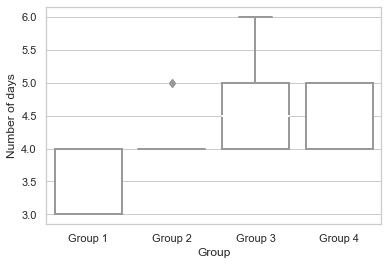
\includegraphics{img/q3_box.png}
    \caption{Side-by-side boxplots}
    \label{fig:q3_box_plot}
\end{figure}

We can observe that the boxplots seem to be similar in shape (except for Group 2, in which the spread is close to that of the others). So our results are acceptable.
\item
Clearly, Treatment technique 1 has smallest average number of days for treatment and is the safest among all the four. Hence, with Treatment 1, space can be managed effectively and at the same time risks can be minimized, and hence, is the one recommended among the four.

\end{enumerate}


\item	Analysis of correlation and regression  \\
\textit{\textbf{Problem:}} \\
%All the \textit{athletes} of IITD participated in a running race trials for Inter-IIT selection, which happened in different time slots (so the distance they ran varied). 

Consider a simple linear regression model with $x$ as predictor variable and $y$ as the response variable. Suppose the following data is obtained from 6 pairs of $x$ and $y$ (the exact data points are not provided):
\[ \sum_{i=1}^{6} x_i = 9.545,
\sum_{i=1}^{6} y_i = 61.668,
\sum_{i=1}^{6} x_i^2 = 15.78468,
\sum_{i=1}^{6} y_i^2 = 719.9573,
\sum_{i=1}^{6} x_i y_i = 96.43722
\]

Let the value of $R^2$ for the linear regression model fitted with the above data be $R_0^2$. Answer the following questions. \textit{Note that the two sub-parts can be solved independent of each other.}

\begin{enumerate}
    \item It was found that a pair $(x,y) = (1.565,3.508)$ was wrong added to the dataset. If the new simple linear regression line equation is of the form $y = b_0' + b_1' x$. Estimate (the numerical values of) $b_0'$ and $b_1'$?
    
    \item Suppose the original regression equation was $y_i = b_0 + b_1x$ and we are interested in multiplying $x$ by a known constant factor $k$ \textit{(scaling)} (for example, conversion of unit from $cm$ to $inches$) and let's call this variable $z$. We can rewrite the above model as $y = b_0^* + b_1^*z$. Find $b_0^*$ and $b_1^*$ in terms of original model parameters ($b_0$ and $b_1$) and $k$? \textbf{What can be said about the value of $R^2$ for this model, in terms of the original one?}
\end{enumerate}

\textit{\textbf{Solution:}} \\

\begin{enumerate}
\item 
Let us calculate the new values. Note that $n$ becomes 5 in this sub-part.

\[ \text{new }  \sum_{i=1}^{5} x_i = 9.545 - 1.565 = 7.98 \]
\[ \text{new } \sum_{i=1}^{5} y_i = 61.668 - 3.508 = 58.16  \]
\[ \text{new } \sum_{i=1}^{5} x_i^2 = 15.78468 - 1.565^2 = 13.33545  \]
\[ \text{new } \sum_{i=1}^{5} y_i^2 = 719.9573 - 3.508^2 = 709.6512 \]
\[ \text{new } \sum_{i=1}^{5} x_i y_i = 96.43722 - (1.565)(3.508) = 90.9472\]

We know the following relation:
\[ b_1' = \frac{S_{xy}}{S_{xx}}, b_0' = \bar y - b_1' \bar x  \]

We now obtain $S_{xx}$ and $S_{xy}$ after the deletion:
\[ S_{xx} = \sum_{i=1}^{n} (x_i-\bar x)^2 = (\sum_{i=1}^{n} x_i^2) - 2 \bar x (\sum_{i=1}^{n} x_i) + n (\bar x)^2 =  (\sum_{i=1}^{n} x_i^2) - \bar x (\sum_{i=1}^{n} x_i)  \]

\[ \implies S_{xx} = 13.33545 - \frac{7.98^2}{5} = 0.59937  \]

On similar lines, 
\[ S_{xy} =  \sum_{i=1}^{n} (x_i - \bar x)(y_i - \bar y) =  (\sum_{i=1}^{n} x_iy_i) - \bar x(\sum_{i=1}^{n} y_i) - \bar y(\sum_{i=1}^{n} x_i) + n\bar x \bar y =  (\sum_{i=1}^{n} x_iy_i) - \frac{(\sum_{i=1}^{n} x_i)(\sum_{i=1}^{n} y_i)}{n} \]

\[ \implies S_{xy} = 90.9472 - \frac{(7.98)(58.16)}{5} =  -1.87616 \].

Plugging the values into $b_1 '$ and $ b_0'$:
\[ b_1 ' = \frac{-1.87616}{0.59937} = -3.13022 \]

\[ b_0' =  \frac{58.16}{5} - (-3.13022)\frac{7.98}{5} = 16.62783 \]

So the new regression equation is $\mathbf{ y = 16.62783 - 3.13022x  }$.


\item
Note that $z = kx$. Using the derivations from part (a), 
\[ b_1^* = \frac{S_{zy}}{S_{zz}} =  \frac{k}{k^2} \frac{ (\sum x_iy_i) - \frac{1}{n}(\sum x_i)(\sum y_i) }{  (\sum x_i^2) - \frac{1}{n}(\sum x_i)^2 } = \frac{1}{k} b_1\]
\[ b_0^* = \bar y - b_1^* k \bar x = \bar y - \frac{1}{k}b_1 k \bar x = b_0  \]

So, the new regression equation is of the form
\[ y = b_0 + \frac{1}{k}b_1z \]

To compute the value of $R^2$:
\[ R^2 = (b_1^*)^2 \frac{S_{zz}}{S_{yy}} = \frac{1}{k^2}(b_1)^2  \frac{k^2 S_{xx}}{S_{yy}} = R_0^2. \]

The $R^2$ value remains the same as the original model.


\end{enumerate}


\item	Analysis of correlation and regression  \\
\textit{\textbf{Problem:}} \\
A coaching institute conducts an admission test for choosing the students for JEE coaching. The institute also gives fee waiver for students who perform well in the test (based on the test scores). 
It is also observed that the fee waiver differ for boys and girls for the same test score by a \textit{constant} value, whose value is not known. %% this quoted in solution
%% It is also observed that this fee waiver percentage varies by a \textit{constant} value between girls and boys, whose value is not known. %% this quoted in solution
Table \ref{tab:q5_boys_data_1} and \ref{tab:q5_girls_data_1} contains the test scores and fee waiver (in \%) for 5 boys and 5 girls who have got admission in that institute.

\begin{table}[h]
    \centering
    \begin{tabular}{l|lllll}
         Test score & 100 & 91 & 85 & 78 & 60 \\ \hline
         Fee Waiver (in \%)&  65& 60& 55& 51& 40 \\
    \end{tabular}
    \caption{Data for boys}
    \label{tab:q5_boys_data_1}
\end{table}

\begin{table}[h]
    \centering
    \begin{tabular}{l|lllll}
         Test score & 97 & 92 & 81 & 73 & 70 \\ \hline
         Fee Waiver (in \%)&  68& 65&  58&  53& 51 \\
    \end{tabular}
    \caption{Data for girls}
    \label{tab:q5_girls_data_1}
\end{table}

You are interested in making a single linear regression model to predict the fee waiver based on test score and gender. 

\begin{enumerate}
    \item Find the least square regression equation for the setup mentioned above? %Clearly mention the units of the coefficients.
    \item You know a boy and a girl who have scored 90 marks in the admission test. Find the estimated fee waiver for each of them?
    %\item Compute the coefficient of linear multiple determination of fee waiver on test score and gender?
    \item Compute the proportion of variation in fee waiver that can be explained by both test score and gender together?
    %\item Compute the coefficients of linear partial correlation?
    \item For a constant test score, how are fee waiver and gender co-related? Quantify it?
    \item Plot a scatter plot for the given data for each gender on the same plot? \textit{Use different colours or markers to differentiate between them.} Given that the fee waiver differs by a constant amount for boys and girls for the same test score, how would you expect the regression line to be (ideally)? \textit{You do not have to solve for the best parameters for the regression line.}
    
\end{enumerate}


%x = np.array([ [0,100], [0,91], [0,85], [0,78], [0,60], [1,97], [1,92], [1,70], [1,81], [1,73]  ])
%#print((lambda x: 2 + 0.63*x)(x))
%y = np.array([ 65, 60, 55, 51, 40, 68, 65, 51, 58,  53 ])

\textit{\textbf{Solution:}} \\
Since it is given that "\textit{fee waiver differ for boys and girls for the same test score by a \textit{constant} value}"
%fee waiver percentage varies by a \textit{constant} value between girls and boys
and since this value is unknown (to be estimated), we can use an indicator variable  to denote gender, whose value will be $1$ for girl and $0$ for boy, so that the extra constant value will get included accordingly.

Let $Y$ denote the fee waiver (in \%), $X_1$ denote the gender (indicator variable defined above) and $X_2$ denote the test score. We can rewrite the given data as in Table \ref{tab:q5_upd_data_1}.

\begin{table}[h]
    \centering
    \begin{tabular}{l|llllllllll}
         Gender ($\mathbf{X_1}$) & 0 & 0 & 0 & 0 & 0 & 1 & 1 & 1 & 1 & 1 \\ \hline
         Test score ($\mathbf{X_2}$)  & 100 & 91 & 85 & 78 & 60 & 97 & 92 & 81 & 73 & 70 \\ \hline
         Fee Waiver (in \%) ($\mathbf{Y}$)&  65& 60& 55& 51& 40  & 68& 65&  58&  53& 51\\
    \end{tabular}
    \caption{Rewritten data which includes the gender indicator variable}
    \label{tab:q5_upd_data_1}
\end{table}

\begin{enumerate}
\item 
The general form of the multiple linear regression can be written as:
\[ Y = b_0 + b_1X_1 + b_2X_2 \]
The normal equations for least square fitting method are (where $N=10$):


\[ \sum Y = b_0N + b_1 \sum X_1 + b_2\sum X_2 \]
\[ \sum YX_1 = b_0 \sum X_1 + b_1 \sum X_1^2 + b_2 \sum X_1X_2 \]
\[ \sum YX_2 = b_0 \sum X_2 + b_1 \sum X_1X_2 + b_2 \sum X_2^2 \]

Substituting the values from Table \ref{tab:q5_upd_data_1}, we get the following system of linear equations:

\[ 566 = 10 b_0 + 5 b_1  + 827 b_2 \]
\[ 295 = 5 b_0 + 5 b_1 + 413 b_2  \]
\[ 47726 = 827 b_0 + 413 b_1 + 69853 b_2 \]

Solving the above system gives
\[ b_0 = 2.01331507, b_1 = 4.92605479, b_2 = 0.63027397 \]

Hence, the required regression equation of $Y$ on $X_1$ and $X_2$ is:
\[\mathbf{ Y = 2.013 + 4.926 X_1 + 0.63 X_2 }\]

% array([2.01331507, 4.92605479, 0.63027397])

\item
\begin{enumerate}
    \item To get the estimated fee waiver for a boy whose test score is 90 in the admission test, we substitute $X_1 = 0$ and $X_2 = 90$. We get the estimated fee waiver as $\mathbf{58.713\%}$.
    
    \item To get the estimated fee waiver for a girl whose test score is 90 in the admission test, we substitute $X_1 = 1$ and $X_2 = 90$. We get the estimated fee waiver as $\mathbf{63.639\%}$.
\end{enumerate}

\item
The proportion of variation in fee waiver that can be explained by test score and gender is measured by coefficient of linear multiple determination.

The standard error of estimate is $\sqrt{\frac{\sum (Y-Y_{est})^2}{N}} = 0.2867$.
The variance of $Y$ is $63.84$.

Hence, coefficient of linear multiple determination of fee waiver on test score and gender, denoted by $R^2$, is given by ${1-\frac{0.2867^2}{63.8}} = 0.999$.


\item 
%If we keep the constant test score, how are fee waiver and gender co-related? Quantify it?
In this case, we need to find the partial correlation coefficient between fee waiver ($Y$) and gender ($X_1$).

The partial correlation coefficient between $Y$ and $X_1$ is given by $\dfrac{r_{YX_1}-r_{YX_2}r_{X_1X_2} } { \sqrt{ (1-r_{YX_2}^2)(1-r_{X_1X_2}^2) } } = \dfrac{0.3003 -(0.9506)(-0.0082) }  { \sqrt{ (1-(0.9506)^2)(1-(-0.0082)^2) } } = 0.993$.

% r12,r13,r23 = (0.30037570459305535, 0.9506273690628858, -0.008275775473908257)
% 0.9932936042454843

\item
The required scatter plot is given in Figure \ref{fig:q5_scatter_1}. 
\begin{figure}[h]
    \centering
    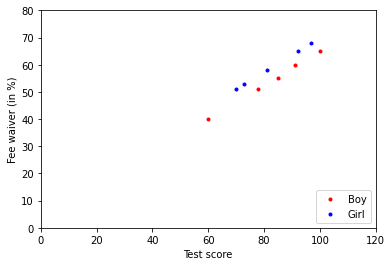
\includegraphics{img/q5_scatter.png}
    \caption{Scatter plot}
    \label{fig:q5_scatter_1}
\end{figure}

As the "\textit{fee waiver differ for boys and girls for the same test score by a \textit{constant} value}", ideally we expect the regression lines which are fitted separately for each gender to have the same slope (parallel) and the difference in y-intercept values would give the difference in fee waiver between boys and girls for the same test score.

\end{enumerate}




\item	Time Series Analysis \\
\textit{\textbf{Problem:}} \\

Consider the following process:
\[ S_t = \frac{7}{5} S_{t-1} - \frac{12}{25} S_{t-2} + \epsilon_t - \frac{9}{5} \epsilon_{t-1} + \frac{4}{5} \epsilon_{t-2} \]

\begin{enumerate}
    \item Classify the above process? \textit{(Note that the process might not be in its minimal form!)}
    \item Is the process stationary? Is it invertible?
    \item Determine $\rho_1$ and $\rho_2$?
\end{enumerate}

\textit{\textbf{Solution:}} \\

\begin{enumerate}
\item 

The given process can be re-written as:
\[ S_t -\frac{7}{5} S_{t-1} + \frac{12}{25} S_{t-2} = \epsilon_t - \frac{9}{5} \epsilon_{t-1} + \frac{4}{5} \epsilon_{t-2} \]

It is a ARMA($p$,$q$) process (where $p$,$q$ are to be found out). For the AR($p$) part, we can express it as ($\mathbb{L}$\ denotes the lag operator):

\[ 1 - \frac{7}{5} \mathbb{L} + \frac{12}{25} \mathbb{L}^2 = 0 \]
\[ \implies \bigg(1 - \frac{3}{5}\mathbb{L} \bigg) \bigg(1- \frac{4}{5}\mathbb{L}  \bigg) = 0  \] 

Similarly, MA($q$) part can be expressed as:
\[ 1 - \frac{9}{5}\mathbb{L} + \frac{4}{5} \mathbb{L}^2 = 0 \]
\[ \implies \bigg(1 - \mathbb{L} \bigg) \bigg(1- \frac{4}{5}\mathbb{L}  \bigg) = 0  \] 

Combining, we have:
\[ \bigg(1 - \frac{3}{5}\mathbb{L} \bigg) \bigg(1- \frac{4}{5}\mathbb{L}  \bigg)S_t = \bigg(1 - \mathbb{L} \bigg) \bigg(1- \frac{4}{5}\mathbb{L}  \bigg) \epsilon_t \]

We have a pair of identical eigenvalues in the two processes. Hence, the given ARMA($p$,$q$) was over-parameterized, which can be reduced to:
\[ \bigg(1 - \frac{3}{5}\mathbb{L} \bigg) S_t = \bigg(1 - \mathbb{L} \bigg) \epsilon_t \]

Or,
\[ S_t =  \frac{3}{5}S_{t-1} + \epsilon_t -  \epsilon_{t-1} \]

This is a \textbf{ARMA(1,1)} process.

\item
\begin{enumerate}
\item 

We know that MA(1) model is stationary by definition. The AR(1) part is also stationary because the root of the characteristic polynomial, which is $\big(1 - \frac{3}{5}z \big ) = 0$, is $5/3$ and $|5/3|>1$ (i.e., it's root lies outside the unit circle). Hence the given process is stationary.
\item
The MA(1) part is not invertible as $1$ is a root of its characteristic polynomial, which is $\big(1 - z \big) = 0$ (not greater than 1). Hence the given process is not invertible.
\end{enumerate}
\item
For ARMA(1,1) process, $\rho_1 = \frac{(1-\phi_1\theta_1)(\phi_1-\theta_1) }{1+\theta_1^2 -2\phi_1\theta_1}$. We have $\phi_1 =  \frac{3}{5}$ and $\theta_1 = -1$. Hence, $\rho_1=0.8$.

Similarly, $\rho_2 = \phi_1\rho_1 = 0.48$.

%For MA($\infty$) representation for the given ARMA(1,1) process:
%\[ \frac{\theta(\mathbb{L})}{\phi(\mathbb{L})} = \frac{1-\mathbb{L}}{1+\frac{3}{5}\mathbb{L}} =
%(1-\mathbb{L})\bigg(1+\frac{3}{5}\mathbb{L} + \Big(\frac{3}{5}\Big)^2\mathbb{L}^2 + \Big(\frac{3}{5}\Big)^3\mathbb{L}^3 + \dots  \bigg)
%\]

%where the last step comes from Taylor series expansion. Simplifying further, we get the above expression as:
%\[
%1 + (1-\frac{3}{5})\mathbb{L} + (1-\frac{3}{5})\frac{3}{5}\mathbb{L}^2 + (1-\frac{3}{5})(\frac{3}{5})^2 \mathbb{L}^2 + \dots 
%\] 



\end{enumerate}

\item[Note: ] All numbers in the data are for illustrative purposes only and might not reflect true numbers from the real-world.

\end{enumerate}



\end{document}
